%\documentclass[A4,12pt]{article}
\documentclass[letterpaper,12pt]{article}
\usepackage{epsfig}
\usepackage{float}
\usepackage{amssymb,amsmath,latexsym}
\usepackage[labelformat=empty]{caption}
\usepackage{color}
%\usepackage[abs]{overpic}

\usepackage{graphicx}
\usepackage{epstopdf}

\usepackage{tikz}
\usetikzlibrary{arrows}
\usetikzlibrary{calc}
\usetikzlibrary{scopes}
\usetikzlibrary{shadows}
\usetikzlibrary{chains}
%\usetikzlibrary{shadows.blur}

\topmargin      0in 
\textheight     9.0in 
\headheight     -0.0in 
\headsep        0in
\textwidth      6.5in 
\oddsidemargin  0in 
\evensidemargin 0in
\parskip        0pt

\newcommand{\slfrac}[2]{\left.#1\middle/#2\right.}
\newcommand{\bm}    [1]{\mbox{\boldmath $#1$}}

\newtheorem{thm}           {Theorem}
\newtheorem{lemma}    [thm]{Lemma}
\newtheorem{prop}     [thm]{Proposition}
\newtheorem{property} [thm]{Property}
\newtheorem{defin}    [thm]{Definition}
\newtheorem{corollary}     {Corollary}

\begin{document}

  %--------------------------------------------------------------
  \begin{enumerate}
    \item[{\bf 6. }]  \textbf{Biased vs. Unbiased estimation} \hfill \\
    \begin{itemize}
      \item[(a)] We first generate stationary gaussian samples $\{x(n)\}_{n=0}^{M-1}$ with $M = 100$.
      Then we use the following formula to estimate the autocorrelation for $-M+1 \leq m \leq M-1$
      \begin{eqnarray*}
        r_{unbiased}(m) & = & \frac{1}{M - |m|} \sum_{n=0}^{M - |m| - 1} x(n)x(n + |m|) \\
        r_{biased}(m)   & = & \frac{1}{M} \sum_{n=0}^{M - |m| - 1} x(n)x(n + |m|). 
      \end{eqnarray*}
      The estimations are shown below
      \begin{figure}[H]
        \centering
        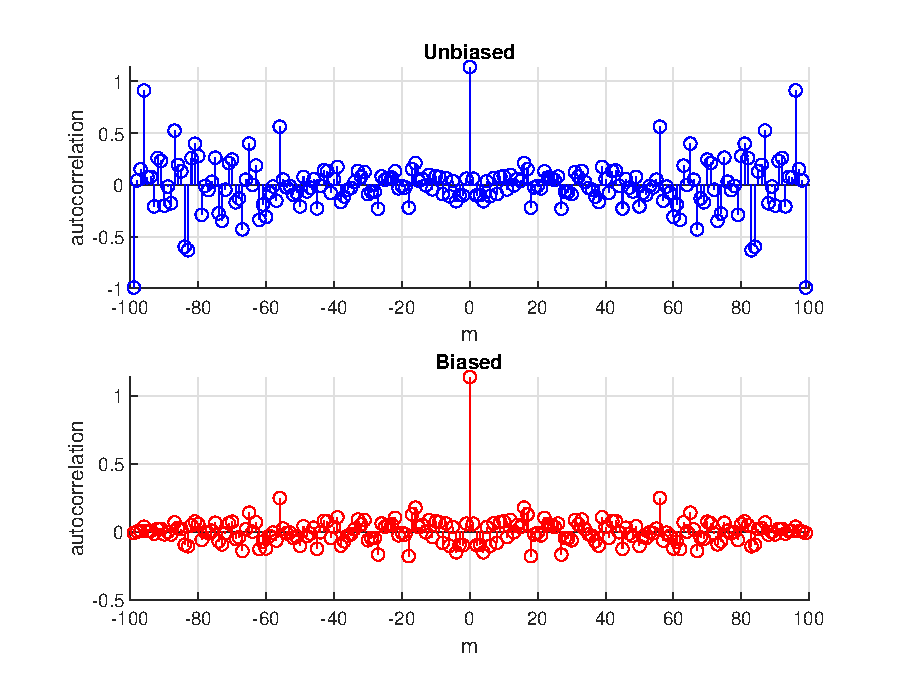
\includegraphics[scale = 1.0]{autocorrelation.eps}
        \caption{Figure 1. Biased and Unbiased estimation}
      \end{figure}
      \textcolor{blue}{It can be seen that the unbiased estimator has higher variance for $m > \frac{M}{4} = 25$.}
      \item[(b)] We first find the correlation matrix $R_{25}$ and $R_{100}$ formed by results of 
      biased and unbiased estimator we obtain in (a). Then we \textcolor{blue}{check the eigenvalues of each correlation matrix.}
      \begin{figure}[H]
        \centering
        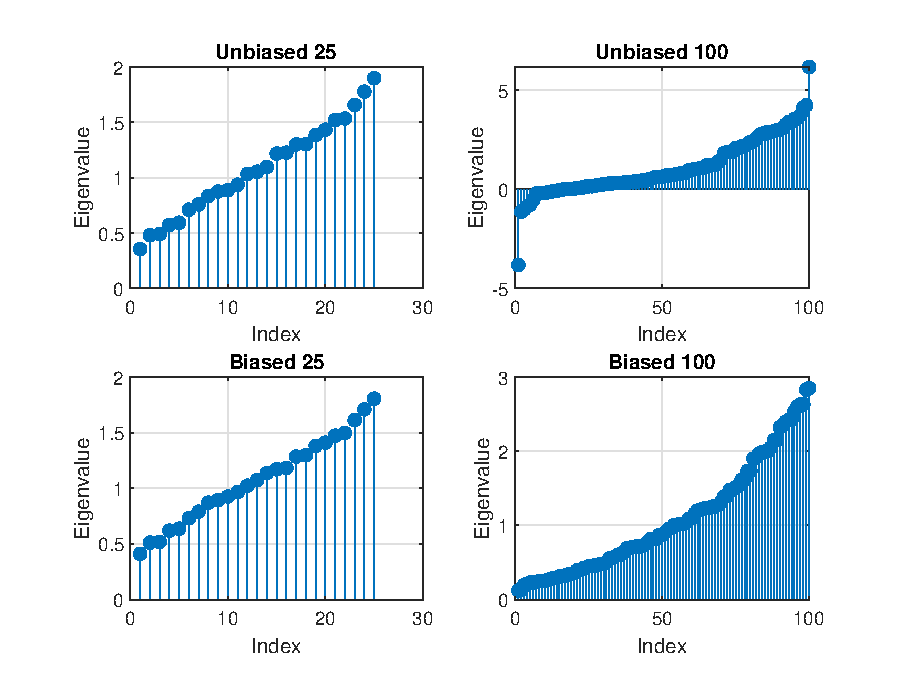
\includegraphics[scale = 1.0]{Rxx.eps}
      \end{figure}
      It can be seen that for $M = 25$, the correlation matrixs formed by the results of both estimator are PSD (Positive Semi-Definite). 
      \textcolor{blue}{For $M = 100$, the correlation matrix formed by the results of unbiased estimator is not PSD since there are negative eigenvalues.}
      In the following, we will prove that \textcolor{blue}{the correlation matrix formed by the results of the biased estimator is always PSD.} \hfill \\
      \hfill \\
      Consider a random signal $\{x(n)\}_{n=0}^{M-1}$. Suppose we want to estimate a $K \times K$ correlation matrix. Let 
      \begin{equation*}
        X = \left(\begin{array}{cccc}
          x[0] & 0 & \hdots & 0 \\
          x[1] & x[0] & \hdots & 0 \\
          \vdots & \vdots & \ddots & \vdots \\
          x[K-1] & x[K-2] & \hdots & x[0] \\
          \vdots & \vdots & \ddots & \vdots \\
          x[M-1] & x[M-2] & \hdots & x[M-P] \\
          0 & x[M-1] & \hdots & x[M - P - 1] \\
          \vdots & \vdots & \ddots & \vdots \\
          0 & 0 & \hdots & [M-1]
        \end{array}\right).
      \end{equation*}
      Then the correlation matrix of biased estimator is given by
      \begin{equation*}
        R_P = \frac{1}{M} X^{H}X
      \end{equation*}
      It can be seen that
      \begin{equation*}
        R(k, l) = \frac{1}{M} \sum_{n=0}^{M - |k-l| - 1} x(n)x(n + |k-l|) = r_{biased}(|k - l|)
      \end{equation*}
      Therefore, \textcolor{blue}{$R$ is a Toeplitz matrix formed by $\{r_{biased}(m)\}_{m=0}^{M-1}$.} For any vector $a$, we have
      \begin{equation*}
        a^HRa = \frac{1}{M}a^HX^HXa = \frac{1}{M} \|Xa\|^2 \geq 0
      \end{equation*}
      Therefore, the correlation matrix formed by the results of the biased estimator is always PSD.
    \end{itemize}
  \end{enumerate}
  
\end{document}
